\begin{frame}
    \frametitle{Discrete Event Simulation - M|M|1}
    \centering

    \begin{figure}[h]
        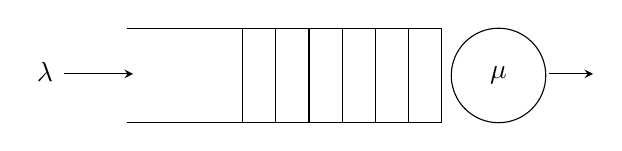
\begin{tikzpicture}[>=stealth, scale=0.8] 
            \draw (2,1.25) -- ++(5cm,0) -- ++(0,-1.5cm) -- ++(-5cm,0);
            \foreach \i in {1,...,6}
            \draw (7cm-\i*15pt,1.25) -- +(0,-1.5cm);
            \draw (7.9,0.5) circle [radius=0.75cm];
            \node[] at (0.7, 0.55) {$\lambda$};
            \draw[->] (1, 0.525) -- (2.1, 0.525);
            \node[] at (7.9,0.5) {$\mu$};
            \draw[->] (8.7,0.525) -- +(20pt,0);
        \end{tikzpicture}
    \end{figure}
\end{frame}    


\begin{frame}
    \frametitle{Discrete Event Simulation - M|M|3}
    \centering
    \begin{figure}[h]
        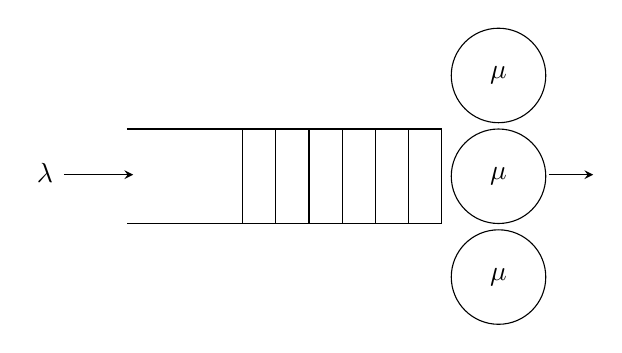
\begin{tikzpicture}[>=stealth, scale=0.8] 
            \draw (2,1.25) -- ++(5cm,0) -- ++(0,-1.5cm) -- ++(-5cm,0);
            \foreach \i in {1,...,6}
            \draw (7cm-\i*15pt,1.25) -- +(0,-1.5cm);
            \draw (7.9,-1.1) circle [radius=0.75cm];
            \node[] at (7.9,-1.1) {$\mu$};
            \draw (7.9,0.5) circle [radius=0.75cm];
            \node[] at (7.9,0.5) {$\mu$};
            \draw (7.9,2.1) circle [radius=0.75cm];
            \node[] at (7.9,2.1) {$\mu$};
            \node[] at (0.7, 0.55) {$\lambda$};
            \draw[->] (1, 0.525) -- (2.1, 0.525);
            \draw[->] (8.7,0.525) -- +(20pt,0);
        \end{tikzpicture}
    \end{figure}
\end{frame}


\begin{frame}
    \frametitle{Discrete Event Simulation - Network of queues}
    \centering
    \begin{figure}[h]
        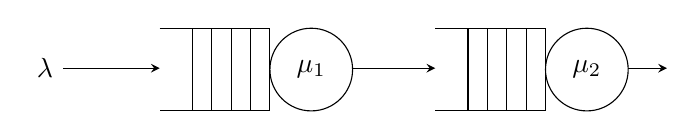
\begin{tikzpicture}[>=stealth, scale=0.7]
            % the first rectangle with vertical lines
            \draw (0,1.25) -- ++(2cm,0) -- ++(0,-1.5cm) -- ++(-2cm,0);
            \foreach \i in {1,...,4}
            \draw (2cm-\i*10pt,1.25) -- +(0,-1.5cm);
            
            % the first circle
            \draw (2.75, 0.5cm) circle [radius=0.75cm];
            \node[align=center] at (2.75cm, 0.5cm) {\( \mu_1 \)};
    
            % the second rectangle with vertical lines
            \draw (5,1.25) -- ++(2cm,0) -- ++(0,-1.5cm) -- ++(-2cm,0);
            \foreach \i in {1,...,4}
            \draw (7cm-\i*10pt,1.25) -- +(0,-1.5cm);

            % the second circle
            \draw (7.75,0.5) circle [radius=0.75cm];
            \node[align=center] at (7.75cm, 0.5cm) {\( \mu_2 \)};
    
            % the arrows and labels (Queue 1+2)
            \draw[->] (8.5, 0.525) -- +(20pt,0);
            \draw[<-] (0, 0.525) -- +(-50pt,0) node[left] {\( \lambda \)};
            \draw[->] (3.5, 0.525) -- (5, 0.525);

        \end{tikzpicture}
    \end{figure}
\end{frame}


\begin{frame}
    \frametitle{Discrete Event Simulation - Custom network}
    \centering
    \begin{figure}[h]
        \begin{tikzpicture}[>=stealth, scale=0.7] %arrow type
            % Queue 1
            \draw (1,0) -- ++(2cm,0) -- ++(0,-1.5cm) -- ++(-2cm,0);
            \foreach \i in {1,...,4}
            \draw (3cm-\i*10pt,0) -- +(0,-1.5cm);
            % \draw (2.75,-0.75cm) circle [radius=0.75cm];
                
            % Queue 2
            \draw (5,1.25) -- ++(2cm,0) -- ++(0,-1.5cm) -- ++(-2cm,0);
            \foreach \i in {1,...,4}
            \draw (7cm-\i*10pt,1.25) -- +(0,-1.5cm);
            \draw (7.75,0.5) circle [radius=0.75cm];

            % The two vertical lines at the very start of Queue 2 
            \draw (7cm-54pt,1.2) -- +(0,-0.5cm);
            \draw (7cm-54pt,0.3) -- +(0,-0.5cm);        
            \draw (7cm-51pt,1.1) -- +(0,-0.4cm);
            \draw (7cm-51pt,0.3) -- +(0,-0.4cm);
            \node[anchor=north] at (5.15, 0.83 cm) {\scriptsize{T}};
        
            % the arrows and labels (Queue 1+2)
            \node[align=center] at (1cm,-2cm) {};
            \node[align=center] at (6cm,-0.75cm) {};
            
            % Arrows lines
            \draw (4.2, 1.8) -- +(-5.2,0) node[left] {\( \lambda_1 \)};
            \draw[<-] (1,-0.75) -- +(-2,0) node[left] {\( \lambda_2 \)};
            \draw[->] (4.2, 0.525) -- (5, 0.525);
            \draw[->] (8.5,0.525) -- (9.3,0.525);
            
            % Others lines
            \draw[-] (3,-0.75) -- (4.2,-0.75);
            \draw (4.2, 0.525) -- (4.2, -0.75);
            \draw (4.2, 1.8) -- (4.2, 0.525);

        \end{tikzpicture}
    \end{figure}
\end{frame}
